\documentclass[tikz]{standalone}
\usepackage{pgfplots}
\pgfplotsset{compat=1.15}
\usepackage{mathrsfs}
\usetikzlibrary{arrows,calc}
\usepackage{tkz-euclide}

\usepackage{fp}
\pagestyle{empty}

\definecolor{AngleClr}{rgb}{0,0.39215686274509803,0}
\definecolor{ShapeClr}{rgb}{0.6,0.2,0}

\begin{document}

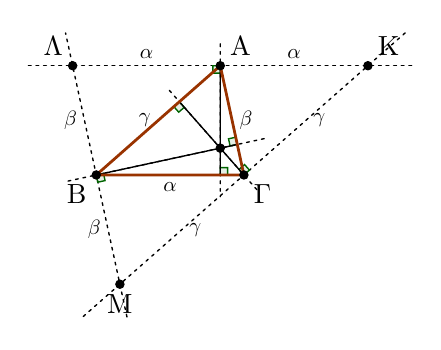
\begin{tikzpicture}[scale=.75]
\tkzSetUpLine[line width=1pt,color=black]
\tkzSetUpPoint[fill=black]

\tkzDefPoints{0/0/L,0.8/-3.7/M,5/0/K}

\tkzDefMidPoint(M,L) \tkzGetPoint{B}
\tkzDefMidPoint(L,K) \tkzGetPoint{A}
\tkzDefMidPoint(K,M) \tkzGetPoint{C}

\tkzDefTriangleCenter[ortho](A,C,B)\tkzGetPoint{H}

\tkzDefPointBy[projection=onto C--B](H)\tkzGetPoint{HA}
\tkzDefPointBy[projection=onto A--C](H)\tkzGetPoint{HB}
\tkzDefPointBy[projection=onto A--B](H)\tkzGetPoint{HC}

\tkzDrawSegment[line width=0.5pt,color=black,dashed,dash pattern=on 1pt off 1.75pt,add=0.15 and 0.15](L,K)
\tkzDrawSegment[line width=0.5pt,color=black,dashed,dash pattern=on 1pt off 1.75pt,add=0.15 and 0.15](K,M)
\tkzDrawSegment[line width=0.5pt,color=black,dashed,dash pattern=on 1pt off 1.75pt,add=0.15 and 0.15](M,L)

\tkzDrawSegment[line width=0.5pt,color=black,dashed,dash pattern=on 1pt off 1.75pt,add=0.2 and 0.2](A,HA)
\tkzDrawSegment[line width=0.5pt,color=black,dashed,dash pattern=on 1pt off 1.75pt,add=0.2 and 0.2](B,HB)
\tkzDrawSegment[line width=0.5pt,color=black,dashed,dash pattern=on 1pt off 1.75pt,add=0.2 and 0.2](C,HC)

\tkzMarkRightAngle[line width=0.5pt, size=.125,color=AngleClr,fill=AngleClr,fill opacity=0.1](H,HA,C)
\tkzMarkRightAngle[line width=0.5pt, size=.125,color=AngleClr,fill=AngleClr,fill opacity=0.1](H,HB,A)
\tkzMarkRightAngle[line width=0.5pt, size=.125,color=AngleClr,fill=AngleClr,fill opacity=0.1](H,HC,B)

\tkzMarkRightAngle[line width=0.5pt, size=.125,color=AngleClr,fill=AngleClr,fill opacity=0.1](H,A,L)
\tkzMarkRightAngle[line width=0.5pt, size=.125,color=AngleClr,fill=AngleClr,fill opacity=0.1](H,B,M)
\tkzMarkRightAngle[line width=0.5pt, size=.125,color=AngleClr,fill=AngleClr,fill opacity=0.1](H,C,K)

\tkzDrawSegment[line width=0.5pt,color=black](A,HA)
\tkzDrawSegment[line width=0.5pt,color=black](C,HC)
\tkzDrawSegment[line width=0.5pt,color=black](B,HB)

\tkzDrawPolygon[color=ShapeClr](A,B,C)
\tkzDrawPoints[size=3](A,B,C)
\tkzLabelPoint[above right](A){$\rm A$}
\tkzLabelPoint[below left](B){$\rm B$}
\tkzLabelPoint[below right](C){$\rm \Gamma$}
\tkzLabelSegment[below, scale=0.75](C,B){$\alpha$}
\tkzLabelSegment[right, scale=0.75](A,C){$\beta$}
\tkzLabelSegment[left, scale=0.75](A,B){$\gamma$}

\tkzDrawPoints[size=3](K,L,M)
\tkzLabelPoint[above right](K){$\rm K$}
\tkzLabelPoint[above left](L){$\rm \Lambda$}
\tkzLabelPoint[below](M){$\rm M$}

\tkzDrawPoints[size=3](H)

\tkzLabelSegment[above, scale=0.75](L,A){$\alpha$}
\tkzLabelSegment[above, scale=0.75](A,K){$\alpha$}


\tkzLabelSegment[left, scale=0.75](M,B){$\beta$}
\tkzLabelSegment[left, scale=0.75](B,L){$\beta$}
\tkzLabelSegment[right, scale=0.75](M,C){$\gamma$}
\tkzLabelSegment[right, scale=0.75](C,K){$\gamma$}

\end{tikzpicture}

\end{document}
